\documentclass[a4paper, 14pt]{extarticle}

% Поля
%--------------------------------------
\usepackage{geometry}
\geometry{a4paper,tmargin=2cm,bmargin=2cm,lmargin=3cm,rmargin=1cm}
%--------------------------------------


%Russian-specific packages
%--------------------------------------
\usepackage[T2A]{fontenc}
\usepackage[utf8]{inputenc} 
\usepackage[english, main=russian]{babel}
%--------------------------------------

\usepackage{textcomp}

% Красная строка
%--------------------------------------
\usepackage{indentfirst}               
%--------------------------------------             


%Graphics
%--------------------------------------
\usepackage{graphicx}
\graphicspath{ {./images/} }
\usepackage{wrapfig}
%--------------------------------------

% Полуторный интервал
%--------------------------------------
\linespread{1.3}                    
%--------------------------------------

%Выравнивание и переносы
%--------------------------------------
% Избавляемся от переполнений
\sloppy
% Запрещаем разрыв страницы после первой строки абзаца
\clubpenalty=10000
% Запрещаем разрыв страницы после последней строки абзаца
\widowpenalty=10000
%--------------------------------------

%Списки
\usepackage{enumitem}

%Подписи
\usepackage{caption} 

%Гиперссылки
\usepackage{hyperref}

\hypersetup {
	unicode=true
}

%Рисунки
%--------------------------------------
\DeclareCaptionLabelSeparator*{emdash}{~--- }
\captionsetup[figure]{labelsep=emdash,font=onehalfspacing,position=bottom}
%--------------------------------------

\usepackage{tempora}

%Листинги
%--------------------------------------
\usepackage{listings}
\lstset{
  basicstyle=\ttfamily\footnotesize, 
  %basicstyle=\footnotesize\AnkaCoder,        % the size of the fonts that are used for the code
  breakatwhitespace=false,         % sets if automatic breaks shoulbd only happen at whitespace
  breaklines=true,                 % sets automatic line breaking
  captionpos=t,                    % sets the caption-position to bottom
  inputencoding=utf8,
  frame=single,                    % adds a frame around the code
  keepspaces=true,                 % keeps spaces in text, useful for keeping indentation of code (possibly needs columns=flexible)
  keywordstyle=\bf,       % keyword style
  numbers=left,                    % where to put the line-numbers; possible values are (none, left, right)
  numbersep=5pt,                   % how far the line-numbers are from the code
  xleftmargin=25pt,
  xrightmargin=25pt,
  showspaces=false,                % show spaces everywhere adding particular underscores; it overrides 'showstringspaces'
  showstringspaces=false,          % underline spaces within strings only
  showtabs=false,                  % show tabs within strings adding particular underscores
  stepnumber=1,                    % the step between two line-numbers. If it's 1, each line will be numbered
  tabsize=2,                       % sets default tabsize to 8 spaces
  title=\lstname                   % show the filename of files included with \lstinputlisting; also try caption instead of title
}
%--------------------------------------

%%% Математические пакеты %%%
%--------------------------------------
\usepackage{amsthm,amsfonts,amsmath,amssymb,amscd}  % Математические дополнения от AMS
\usepackage{mathtools}                              % Добавляет окружение multlined
\usepackage[perpage]{footmisc}
%--------------------------------------

%--------------------------------------
%			НАЧАЛО ДОКУМЕНТА
%--------------------------------------

\begin{document}

%--------------------------------------
%			ТИТУЛЬНЫЙ ЛИСТ
%--------------------------------------
\begin{titlepage}
\thispagestyle{empty}
\newpage


%Шапка титульного листа
%--------------------------------------
\vspace*{-60pt}
\hspace{-65pt}
\begin{minipage}{0.3\textwidth}
\hspace*{-20pt}\centering

\includegraphics[width=\textwidth]{emblem}
\end{minipage}
\begin{minipage}{0.67\textwidth}\small \textbf{
\vspace*{-0.7ex}
\hspace*{-6pt}\centerline{Министерство науки и высшего образования Российской Федерации}
\vspace*{-0.7ex}
\centerline{Федеральное государственное бюджетное образовательное учреждение }
\vspace*{-0.7ex}
\centerline{высшего образования}
\vspace*{-0.7ex}
\centerline{<<Московский государственный технический университет}
\vspace*{-0.7ex}
\centerline{имени Н.Э. Баумана}
\vspace*{-0.7ex}
\centerline{(национальный исследовательский университет)>>}
\vspace*{-0.7ex}
\centerline{(МГТУ им. Н.Э. Баумана)}}
\end{minipage}
%--------------------------------------

%Полосы
%--------------------------------------
\vspace{-25pt}
\hspace{-35pt}\rule{\textwidth}{2.3pt}

\vspace*{-20.3pt}
\hspace{-35pt}\rule{\textwidth}{0.4pt}
%--------------------------------------

\vspace{1.5ex}
\hspace{-35pt} \noindent \small ФАКУЛЬТЕТ\hspace{80pt} <<Информатика и системы управления>>

\vspace*{-16pt}
\hspace{47pt}\rule{0.83\textwidth}{0.4pt}

\vspace{0.5ex}
\hspace{-35pt} \noindent \small КАФЕДРА\hspace{50pt} <<Теоретическая информатика и компьютерные технологии>>

\vspace*{-16pt}
\hspace{30pt}\rule{0.866\textwidth}{0.4pt}
  
\vspace{11em}

\begin{center}
\Large {\bf Лабораторная работа № 6.1} \\ 
\large {\bf по курсу <<Компьютерные сети>>} \\
\large <<Разработка SMTP-клиента и приложения почтовой рассылки>> 
\end{center}\normalsize

\vspace{8em}


\begin{flushright}
  {Студент группы ИУ9-32Б Волохов А. В. \hspace*{15pt}\\ 
  \vspace{2ex}
  Преподаватель Посевин Д. П.\hspace*{15pt}}
\end{flushright}

\bigskip

\vfill
 

\begin{center}
\textsl{Москва 2023}
\end{center}
\end{titlepage}
%--------------------------------------
%		КОНЕЦ ТИТУЛЬНОГО ЛИСТА
%--------------------------------------

\renewcommand{\ttdefault}{pcr}

\setlength{\tabcolsep}{3pt}
\newpage
\setcounter{page}{2}
\section{Задание}\label{Sect::task}
Рассматривается задача разработки smtp-клиента на языке Golang.

Используя пакеты https://pkg.go.dev/net/smtp, https://pkg.go.dev/crypto/tls, а также в
зависимости от реализации возможно понадобится https://pkg.go.dev/strings.
Необходимо реализовать задачи приведенные ниже.

Задача 1: SMTP-клиент на Golang.
Необходимо реализовать программу отправки проверочного SMTP
сообщения, которое необходимо производить на ящик danila@bmstu.posevin.ru с
одного из электронных ящиков, доступ к которым приведен ниже. При этом
работоспособность приложения необходимо продемонстрировать очно. В этом
приложении должны быть реализованы следующие функции:
ввод значения поля To из командной строки;
ввод значения поля Subject из командной строки;
вод сообщения в поле Message body из командной строки.
При отправке проверочного сообщения необходимо в теме сообщения
обязательно указать фамилию, имя и группу студента выполнившего задание.

Задача 2: Приложение почтовых рассылок.

1. В базе данных MySQL создать таблицу рассылки, в которой должны быть
следующие поля: имя пользователя, адрес электронной почты
пользователя, сообщение пользователю.

2. Реализовать рассылку по таблице рассылки, при этом в тексте письма
должно быть реализовано персональное обращение к пользователю, текст
письма оформлен в HTML формате, при этом как минимум приветствие
должно быть выделено жирным шрифтом, текст письма курсивом и фон
письма отличаться от белого, рекомендуется прочитать статьи приведенные
ниже о верстке электронных писем для рассылок.

3. Необходимо реализовать логирование ответов от smtp сервера в момент
сеанса связи в таблицу MySQL.

4. Работоспособность приложения необходимо продемонстрировать очно,
поместив в список рассылки ящики danila@posevin.com, posevin@mail.ru,
posevin@bmstu.ru.
Исходный код программы представлен в листингах~\ref{lst:code1}--~\ref{lst:code2}--~\ref{lst:code3}.

\begin{figure}[!htb]
\begin{lstlisting}[language={Go},caption={client.go},label={lst:code1}]
package main
import (
	"bufio"
	"crypto/tls"
	"fmt"
	"net/smtp"
	"os"
	"strings"
)
func main() {
	fmt.Print("Enter address (To): ")
	to := readInput()
	fmt.Print("Enter Subject: ")
	subject := readInput()
	fmt.Print("Enter Message body: ")
	messageBody := readInput()
	username := "dts21@dactyl.su"
	password := "12345678990DactylSUDTS"
	smtpServer := "mail.nic.ru"
	smtpPort := 465
	useSSL := true
	messageSubject := fmt.Sprintf("%s", subject)
	message := fmt.Sprintf("To: %s\r\nSubject: %s\r\n\r\n%s", to, messageSubject, messageBody)
	tlsConfig := &tls.Config{InsecureSkipVerify: !useSSL, ServerName: smtpServer,}
	conn, err := tls.Dial("tcp", fmt.Sprintf("%s:%d", smtpServer, smtpPort), tlsConfig)
	if err != nil { fmt.Println("Error", err) return}
	defer conn.Close()
	auth := smtp.PlainAuth("", username, password, smtpServer)
	client, err := smtp.NewClient(conn, smtpServer)
	if err != nil {fmt.Println("Error", err) return}
	defer client.Quit()
	if err := client.Auth(auth); err != nil {fmt.Println("Error", err) return}
	if err := client.Mail(username); err != nil {fmt.Println("Error", err) return}
	if err := client.Rcpt(to); err != nil {fmt.Println("Error", err) return}
	writer, err := client.Data()
	if err != nil {
		fmt.Println("Error", err)
		return
	}
	defer writer.Close()
	_, err = writer.Write([]byte(message))
	if err != nil {
		fmt.Println("Error", err)
		return
	}
	fmt.Println("Success.")
}
func readInput() string {
	reader := bufio.NewReader(os.Stdin)
	input, _ := reader.ReadString('\n')
	return strings.TrimSpace(input)
}
\end{lstlisting}
\end{figure}

\newpage

\begin{figure}[!htb]
\begin{lstlisting}[language={Go},caption={app.go},label={lst:code2}]
package main

import (
	"crypto/tls"
	"database/sql"
	"fmt"
	_ "github.com/go-sql-driver/mysql"
	"log"
	"net/smtp"
)

type SMTPSettings struct {
	Server   string
	Port     string
	Username string
	Password string
}

type DBSettings struct {
	Host     string
	Database string
	Username string
	Password string
}

type Mail struct {
	To      string
	Subject string
	Body    string
}

type Log struct {
	To          string
	Status      string
	Description string
}

func main() {
	dbSettings := DBSettings{
		Host:     "students.yss.su",
		Database: "iu9networkslabs",
		Username: "iu9networkslabs",
		Password: "Je2dTYr6",
	}

	smtpSettings := SMTPSettings{
		Server:   "mail.nic.ru",
		Port:     "465",
		Username: "dts21@dactyl.su",
		Password: "12345678990DactylSUDTS",
	}

	db, err := sql.Open("mysql", fmt.Sprintf("%s:%s@tcp(%s)/%s", dbSettings.Username, dbSettings.Password, dbSettings.Host, dbSettings.Database))
	if err != nil {
		log.Fatal(err)
	}
	defer db.Close()
\end{lstlisting}
\end{figure}

\newpage
\begin{figure}[!htb]
\begin{lstlisting}[language={Go},caption={app.go - продолжение},label={lst:code3}]
query := "SELECT username, email, message FROM Volokhov_smtp"
	rows, err := db.Query(query)
	if err != nil {
		log.Fatal(err)
	}
	defer rows.Close()

	for rows.Next() {
		var username, email, message string
		if err := rows.Scan(&username, &email, &message); err != nil {
			log.Println(err)
			continue
		}

		htmlBody := fmt.Sprintf(`<html><body><p><strong>%s</strong>,</p><p><em>%s</em></p><p>%s</p></body></html>`, username, message, message)

		err := sendMail(smtpSettings, Mail{
			To:      email,
			Subject: "Volokhov Aleksandr IU9-32B",
			Body:    htmlBody,
		}, db)
		if err != nil {
			log.Println(err)
			continue
		}

		log.Printf("Mail sent to %s\n", email)
	}
}

func sendMail(smtpSettings SMTPSettings, mail Mail, db *sql.DB) error {
	message := fmt.Sprintf("To: %s\r\nSubject: %s\r\nContent-Type: text/html\r\n\r\n%s", mail.To, mail.Subject, mail.Body)

	auth := smtp.PlainAuth("", smtpSettings.Username, smtpSettings.Password, smtpSettings.Server)

	tlsConfig := &tls.Config{
		ServerName: smtpSettings.Server,
	}

	conn, err := tls.Dial("tcp", fmt.Sprintf("%s:%s", smtpSettings.Server, smtpSettings.Port), tlsConfig)
	if err != nil {
		return err
	}
	defer conn.Close()

	client, err := smtp.NewClient(conn, smtpSettings.Server)
	if err != nil {
		return err
	}
	defer client.Close()

	if err := client.Auth(auth); err != nil {
		return err
	}
\end{lstlisting}
\end{figure}

\newpage
\begin{figure}[!htb]
\begin{lstlisting}[language={Go},caption={app.go - продолжение},label={lst:code3}]
if err := client.Mail(smtpSettings.Username); err != nil {
		return err
	}

	if err := client.Rcpt(mail.To); err != nil {
		return err
	}

	w, err := client.Data()
	if err != nil {
		return err
	}
	defer w.Close()

	_, err = w.Write([]byte(message))
	if err != nil {
		return err
	}

	log := Log{
		To:          mail.To,
		Status:      "success",
		Description: "Email sent successfully",
	}
	if err := insertLog(db, log); err != nil {
		fmt.Println("Failed to insert log into the database:", err)
	}

	return nil
}

func insertLog(db *sql.DB, log Log) error {
	_, err := db.Exec("INSERT INTO Volokhov_logs (to_email, status, description) VALUES (?, ?, ?)", log.To, log.Status, log.Description)
	return err
}
\end{lstlisting}
\end{figure}

\newpage

\begin{figure}[!htb]
	\centering
	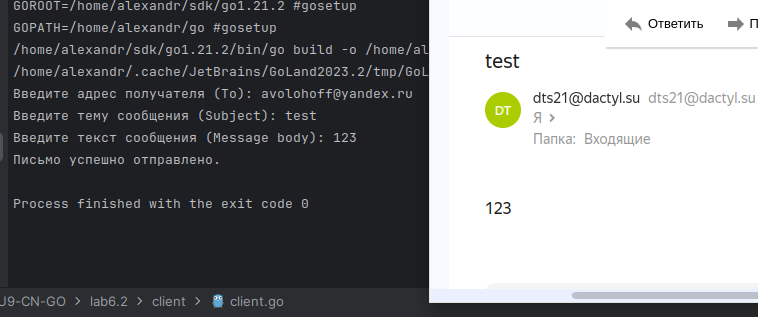
\includegraphics[width=0.8\textwidth]{res1.png}
\caption{Клиент и письмо}
\label{fig:img1}
\end{figure}

\begin{figure}[!htb]
	\centering
	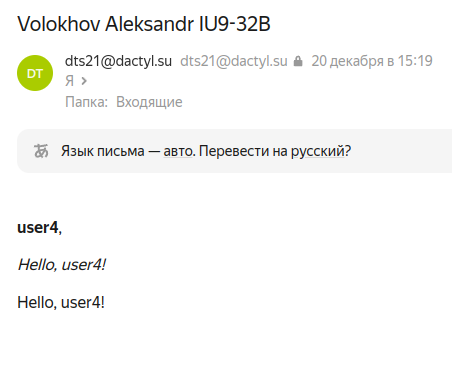
\includegraphics[width=0.8\textwidth]{res2.png}
\caption{Пример письма из рассылки}
\label{fig:img2}
\end{figure}

\begin{figure}[!htb]
	\centering
	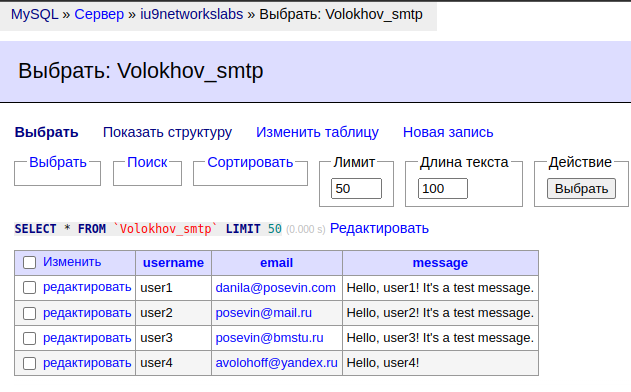
\includegraphics[width=0.8\textwidth]{res3.png}
\caption{База данных рассылки}
\label{fig:img3}
\end{figure}

\begin{figure}[!htb]
	\centering
	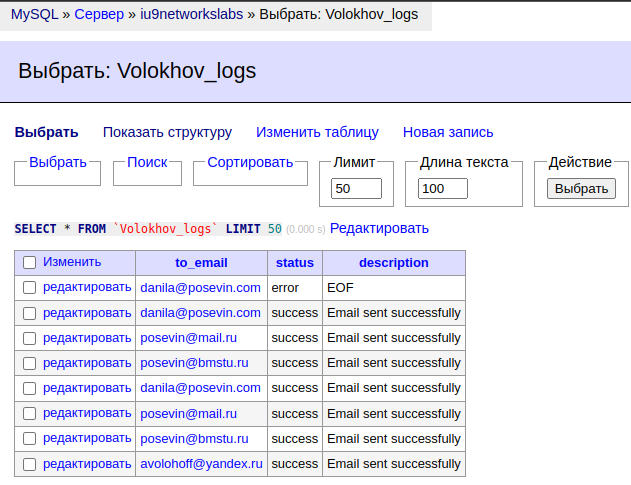
\includegraphics[width=0.8\textwidth]{res4.png}
\caption{База данных логов}
\label{fig:img3}
\end{figure}





\end{document}
